\documentclass[a4paper]{article}

\usepackage{color}
\usepackage{xurl}
\usepackage[T2A]{fontenc} % enable Cyrillic fonts
\usepackage[utf8]{inputenc} % make weird characters work
\usepackage{csquotes}
\usepackage{graphicx}
\usepackage{subfigure}
\usepackage{float}
\usepackage[english,serbian]{babel}
\usepackage{listings}
\usepackage{amsthm}
\usepackage{amsmath}

\usepackage[unicode]{hyperref}
\hypersetup{colorlinks,citecolor=green,filecolor=green,linkcolor=blue,urlcolor=blue}

\newtheorem{theorem}{Theorem}[section]
\newtheorem{lemma}[theorem]{Lema}

\title{\textit{Beam Stack Search} algoritam pretrage u okviru alata za simboličko izvršavanje KLEE\\ \small{Seminarski rad u okviru kursa\\Verifikacija softvera\\Matematički fakultet}}
\author{Aleksandar Stefanović, 1021/2023 \and Petar Đorđević, 1088/2022}

\begin{document}

\maketitle

\begin{abstract}

\end{abstract}

\tableofcontents

\newpage

\section{Uvod}

Simboličko izvršavanje u svom osnovnom obliku predstavlja tehniku statičke verifikacije programa, tj. verifikacije programa bez njegovog pokretanja, u kojoj se umesto konkretnog stanja programa tokom izvršavanja prati njegovo simboličko stanje \cite{SymExec-King-10.1145/360248.360252}, u cilju otkrivanja grešaka, automatskog generisanja testova sa velikom pokrivenošću koda i slično. Ovo podrazumeva praćenje simboličkih vrednosti promenljivih koje se javljaju u programu, kao i tzv. uslova putanja - logičkih formula nad simboličkim vrednostima tih promenljivih koje moraju da budu zadovoljene da bi izvršavanje stiglo do neke tačke u programu.

Svaka naredba kontrole toka, poput naredbi grananja ili petlji, može prouzrokovati više putanja izvršavanja programa. Ove putanje, zajedno sa pridruženim uslovima putanja i simboličkim vrednostima promenljivih, indukuju simboličko stablo izvršavanja programa. Osim za najtrivijalnije programe, simboličko stablo izvršavanja je nemoguće u potpunosti istražiti. Simboličko stablo izvršavanja program koji sadrži samo $30$ naredbi grananja bi, zanemarujući moguće nedostižne putanje, sadržalo bi $2^{30}$ različitih putanja izvršavanja. Ukoliko program sadrži i petlje, njegovo stablo izvršavanja bi potencijalno bilo i beskonačno veliko (ukoliko i sam uslov prekida petlje ima simboličku vrednost).

Upravo eksplozija broja stanja u simboličkom stablu izvršavanja je jedan od glavnih problema sa kojim se susreću alati za simboličko izvršavanje. Neke od tehnika koje alati koriste da bi umanjili efekat ovog problema su odsecanje nedostižnih putanja, spajanje stanja, zadavanje preduslova i aproksimacija petlji \cite{SurveySymExec-CSUR18}. Međutim, čak i uz primenu ovih tehnika, najčešće nije moguće eliminisati dovoljan broj stanja da bi se efikasno istražilo celokupno simboličko stablo izvršavanja, pa je od velike važnosti izbor stanja, tj. putanja, za ispitivanje.

Izbor narednog stanja za ispitivanje zavisi od primenjene strategije za obilazak puteva. Dve osnovne strategije su \textit{DFS}, tj. pretraga u dubinu, i \textit{BFS}, tj. pretraga u širinu. Iako imaju svoje primene, obe strategije imaju svoje mane - pretraga u dubinu ima tendenciju zaglavljivanja u \enquote{dubokim} putanjama indukovanih petljama ili rekurzijom, dok pretraga u širinu povlači izuzetno veliko memorijsko zauzeće usled potrebe za istovremenim čuvanjem čitavog nivoa čvorova simboličkog stabla izvršavanja. Postoje i hibridne tehnike između ova dva pristupa, poput algoritma \textit{BFS/DFS} \cite{BFS/DFS-StrahinjaStanojevic}. Često se primenjuju i tehnike koje koriste randimozovane varijante algoritama pretrage, gde se stanjima koja imaju neku dobru osobinu može dodeliti prednost prilikom izbora, poput algoritma koji podrazumevano koristi alat za simboličko izvršavanje \verb|KLEE| \cite{KLEE-paper-10.5555/1855741.1855756}.

U nastavku rada će biti predstavljena upotreba \textit{Beam Stack Search} algoritma pretrage, kao i njegova implementacija u okviru alata za simboličko izvršavanje \verb|KLEE|. Na kraju, biće izvršena uporedna analiza performansi ovog algoritma sa nekim od algoritama koje pruža alat \verb|KLEE|.

\section{Opis algoritma}

Algoritam \textit{Beam Stack Search} \cite{BeamStackSearch-10.5555/3037062.3037074} predstavlja proširenje heurističkog algoritma pretrage \textit{Beam Search}, pa će u nastavku prvo biti opisan ovaj algoritam. Iako u opštem slučaju ovi algoritmi imaju mogućnost obilaska proizvoljnog grafa, u nastavku rada će se, zbog potreba u simboličkom izvršavanju, razmatrati samo obilazak stabla.

\subsection{\textit{Beam Search} algoritam pretrage}

Algoritam pretrage \textit{Beam Search}, nadalje \textit{BS} algoritam, svoje najveće primene nalazi u oblasti mašinskog učenja, konkretno u obradi prirodnog jezika i mašinskog prevođenja \cite{HarpySpeechRecognitionSystem, BeamSearchStrategiesForNeuralMachineTranslation, BestFirstBeamSearch}. Međutim, ideje koje on uvodi se mogu primeniti i u simboličkom izvršavanju. Naime, \textit{BS} algoritam, po cenu gubitka kompletnosti pretrage, heurističkim pristupom brzo i uz malu memorijsku potrošnju pronalazi dobre, po nekoj izabranoj metrici, putanje u težinskom grafu. U kontekstu simboličkog izvršavanja, ova ideja se može primeniti na pronalaženje putanja koje, na primer, maksimizuju pokrivenost koda.

Algoritam kao parametar prihvata ceo broj $w$, tj. širinu pretrage, i zasnovan na \textit{BFS} pretrazi, sa modifikacijom da na svakom nivou stabla pretrage zadržava samo $w$ najboljih čvorova (najveće ili najmanje težine, zavisno od izabrane metrike), a ostale čvorove odbacuje. Primer izvršavanja za $w = 2$ nad stablom gde se prednost daje čvorovima veće težine prikazan je na slici \ref{fig:beam_search}. Zeleni čvorovi označavaju čvorove izabrane za pretragu, crveni čvorove koji su odbačeni, a svetlo crveni čvorove koji, kao potomci odbačenih čvorova, nisu ni razmatrani.

\begin{figure}[h!]
    \centering
    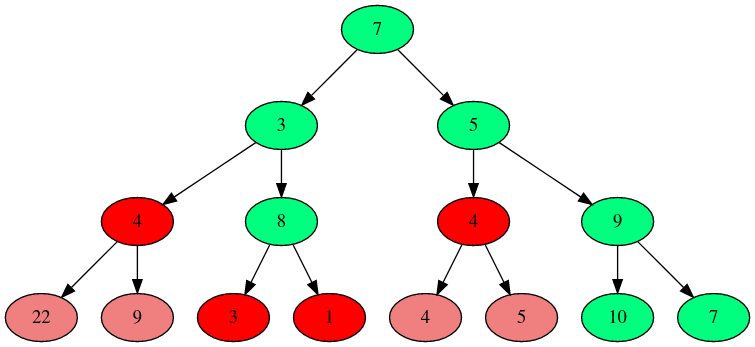
\includegraphics[width=\linewidth]{ilustracije/beam_search_primer.png}
    \caption{Izvršavanje \textit{BS} algoritma nad stablom za širinu pretrage $w = 2$}
    \label{fig:beam_search}
\end{figure}

Pošto se na svakom nivou stabla zadržava samo $w$ čvorova, a prethodno posećeni čvorovi se ne pamte, memorijska složenost ovog algoritma pretrage je $O(w)$, tj. ne zavisi od veličine stabla. Međutim, problem u ovom pristupu je to što će samo $w$ putanja biti u potpunosti (ukoliko su one konačne težine) istraženo, dok su sve ostale putanje odbačene. U kontekstu simboličkog izvršavanja, ovo bi dovelo do gubitka saglasnosti analize. Da bi se ovaj problem rešio, potrebno je izvršiti modifikaciju algoritma, koja je data u vidu \textit{Beam Stack Search} algoritma pretrage.

\subsection{\textit{Beam Stack Search} algoritam pretrage}

\section{Implementacija u okviru alata za simboličko izvršavanje KLEE}

\section{Eksperimentalna evaluacija algoritma}

\section{Zaključak}

\addcontentsline{toc}{section}{Literatura}
\appendix
\bibliography{literatura}
\bibliographystyle{plain}

\end{document}
